\documentclass{article}
\title{Lecture 9 - Inflation and You Calculating CPI}
\author{}
\date{February 6, 2019}
\usepackage[final]{pdfpages}
\usepackage{fullpage}
\usepackage{graphicx}

\begin{document}
\maketitle
\section*{Inflation}
\begin{itemize}
\item Inflation is a continuous increase in price over time.
\item There are two main types of inflation:
    \begin{itemize}
    \item {\bf Demand Pull Inflation}: As demand for a good or set of goods increases, 
       so does its price.
    \item {\bf Cost Push Inflation}: As prices rise, companies must protect their profit
       margin by raising prices.
    \end{itemize}
\item We will discuss the economic causes and implications of inflation in more detail 
  in the next lecture.
\end{itemize}

\section*{Consumer Price Index}
\begin{itemize}
\item Assuming that prices remain roughly proportional, prices can be converted between years.
\item A consumer price index relates average prices to some base year.  These are computed by tracking prices of a selection of goods between two years.
\item The base year is assigned a price index of 100.  The proportional relationship is:
\[
\textrm{price in a given year} : \textrm{price in base year} :: \textrm{CPI for given year} : 100 
\]
\item Discuss:  What relationship does CPI have to percent?
\item For convenience, CPI's are usually standardized to a base year.  All prices are compared to prices on this year.
\item The standard base year, as defined by the United States Bureau of Labor Statistics uses the average prices over the range 1982-1984 as the standard base year.  (This is called a chained base year.)
\item Given the CPI in year a and year b, the following proportion will hold:
\[
\textrm{price in year a} : \textrm{price in year b} :: \textrm{CPI in year a} : \textrm{CPI in year b}
\]
\end{itemize}

\subsection*{Problems and Discussion}
\begin{enumerate}
\item Compute the beef index price based on the 1971 advertisement from A\&P.  
\item Convert the 1971 based beef index to a 1982-1984 based index.  How does this compare to the actual Depart of Labor Statistics CPI for 1971?
\item If a college textbook has a list price of \$12.95 in 1971, what should its price be in 2018?
\item Look up the list price of Hopcroft and Ullman's {\em Introduction to Automata Theory, Languages, and Computation}.  This is the book from the previous question.  Has it kept pace with inflation or has it outperformed it?  What could account for this?
\item Examine the CPI chart for the years 1913-2018.  How does the CPI compare to major events in US history?
\end{enumerate}

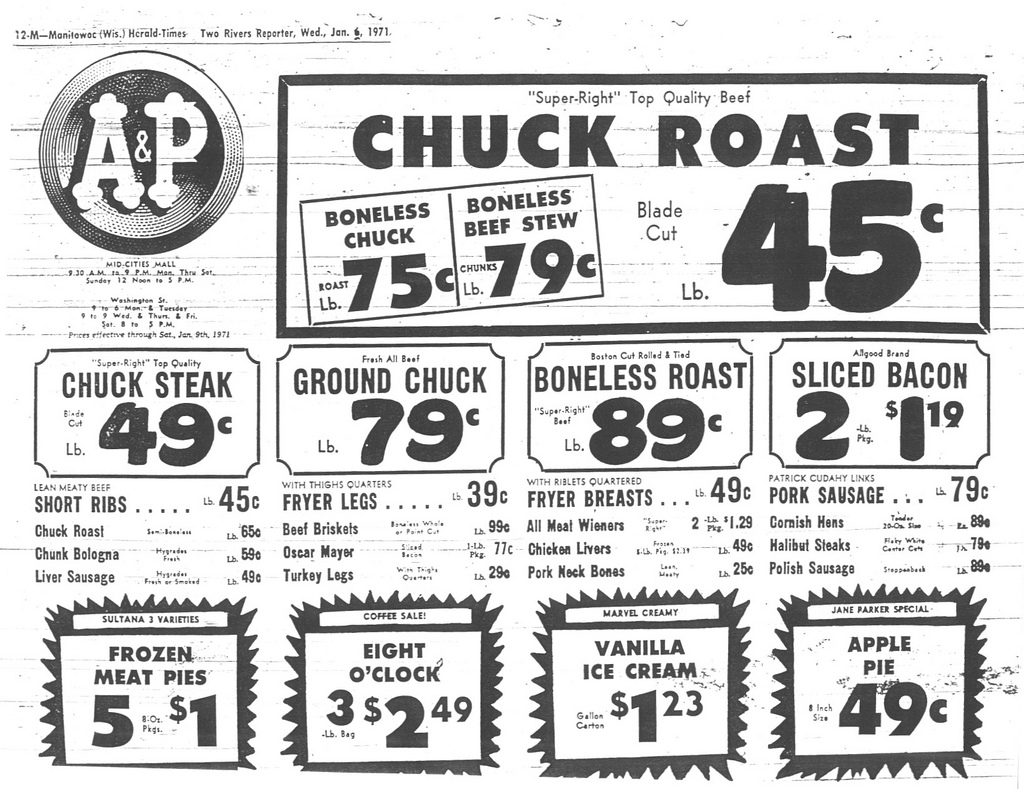
\includegraphics[width=0.9\textwidth]{apfood}\newline
Image Source: {\tt https://www.flickr.com/photos/andrew-turnbull/3347776176}

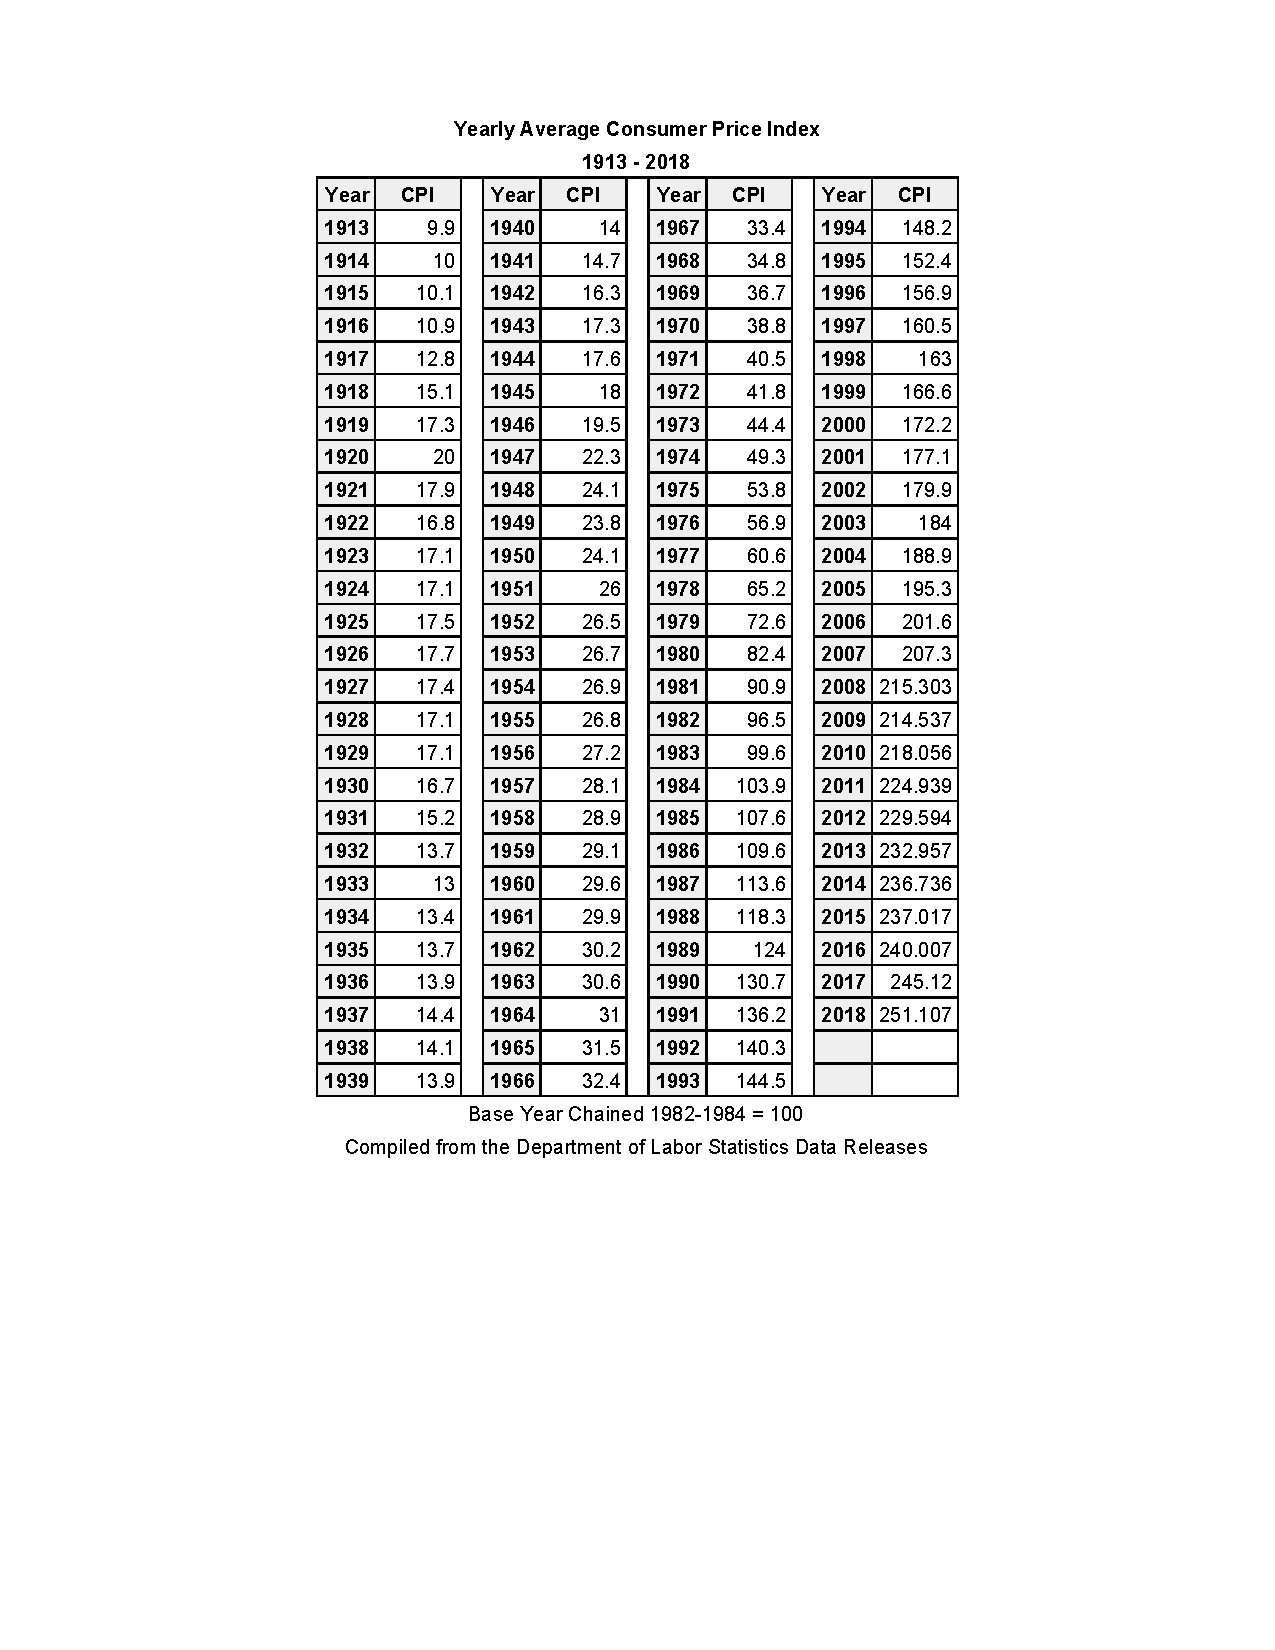
\includepdf[pages=-]{cpi-1913-2018.pdf}
\end{document}
